\icode{E-MD-SI-L2-261114-010}
如图所示，三根在竖直平面内的光滑细管 \(A\)、\(B\)、\(C\) 上端平齐，\(B\) 管竖直放置，\(A\) 管与 \(B\) 管的夹角为 \(\alpha\)，\(C\) 管与 \(B\) 管的夹角为 \(\beta\)，且 \(\alpha > \beta\)。三个小球同时从管口顶端静止释放，经过相同的时间，三球所处位置正确的是\paren[]

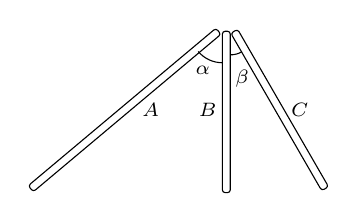
\begin{tikzpicture}[font=\scriptsize]
	\draw (.05,-.3) arc(-90:-60:.3) (-.05,-.4) arc(-90:-140:.4);
	\draw[rounded corners=1] (-.05,0) rectangle(.05,-2.05);
	\draw[rounded corners=1,rotate around={-50:(-.1,0)}] (-.15,0) rectangle(-.05,{-2/cos(50)});
	\draw[rounded corners=1,rotate around={30:(.1,0)}] (.05,0) rectangle(.15,{-2/cos(30)});
	\node at(-.3,-.5){\(\alpha\)};
	\node at(.2,-.6){\(\beta\)};
	\node at(0,-1)[left]{\(B\)};
	\node at(-140:{1/cos(50)})[right]{\(A\)};
	\node at(-55:{1/cos(35)})[right]{\(C\)};
\end{tikzpicture}

\begin{tikzpicture}[scale=.9,font=\scriptsize]
	\begin{scope}
		\draw (.05,-.3) arc(-90:-60:.3) (-.05,-.4) arc(-90:-140:.4);
		\draw[rounded corners=1] (-.05,0) rectangle(.05,-2.05);
    	\draw[rounded corners=1,rotate around={-50:(-.1,0)}] (-.15,0) rectangle(-.05,{-2/cos(50)});
		\draw[rounded corners=1,rotate around={30:(.1,0)}] (.05,0) rectangle(.15,{-2/cos(30)});
		\node at(-.3,-.5){\(\alpha\)};
		\node at(.2,-.6){\(\beta\)};
		\fill[rotate around={-50:(-.1,0)}] (-.1,{-1.5/cos(50)})coordinate(a) circle(.05);
		\fill[rotate around={30:(.1,0)}] (.1,{-1.5/cos(30)}) circle(.05)coordinate(b);
		\fill (0,-1.5) circle(.05);
		\draw[dashed,gray] (a)--(b);
		\node at(-.5,-2.4){\normalsize\(A\)};
	\end{scope}
	\begin{scope}[xshift=4cm]
		\draw (.05,-.3) arc(-90:-60:.3) (-.05,-.4) arc(-90:-140:.4);
		\draw[rounded corners=1] (-.05,0) rectangle(.05,-2.05);
		\draw[rounded corners=1,rotate around={-50:(-.1,0)}] (-.15,0) rectangle(-.05,{-2/cos(50)});
		\draw[rounded corners=1,rotate around={30:(.1,0)}] (.05,0) rectangle(.15,{-2/cos(30)});
		\node at(-.3,-.5){\(\alpha\)};
		\node at(.2,-.6){\(\beta\)};
		\draw[dashed,gray] (-140:1.5) arc(-140:-60:1.5);
		\fill[rotate around={-50:(-.1,0)}] (-.1,-1.42) circle(.05);
		\fill[rotate around={30:(.1,0)}] (.1,-1.45) circle(.05);
		\fill (0,-1.5) circle(.05);
		\node at(-.5,-2.4){\normalsize\(B\)};
	\end{scope}
	\begin{scope}[xshift=8cm]
		\draw (.05,-.3) arc(-90:-60:.3) (-.05,-.4) arc(-90:-140:.4);
		\draw[rounded corners=1] (-.05,0) rectangle(.05,-2.05);
		\draw[rounded corners=1,rotate around={-50:(-.1,0)}] (-.15,0) rectangle(-.05,{-2/cos(50)});
		\draw[rounded corners=1,rotate around={30:(.1,0)}] (.05,0) rectangle(.15,{-2/cos(30)});
		\node at(-.3,-.5){\(\alpha\)};
		\node at(.2,-.6){\(\beta\)};
		\fill (0,-1.5)coordinate(o) circle(.05);
		\draw[dashed,gray] (o)--++(130:{1.5*sin(50)})coordinate(c) (o)--++(30:{1.5*sin(30)})coordinate(d);
		\draw[gray] ($(c)+(-50:.1)$)--++(-140:.1)--++(130:.1) ($(d)+(-150:.1)$)--++(-60:.1)--++(30:.1);
		\fill[rotate around={-50:(-.1,0)}] (-.1,{-1.5*cos(50)+.05}) circle(.05);
		\fill[rotate around={30:(.1,0)}] (.1,{-1.5*cos(30)+.03}) circle(.05);
		\node at(-.5,-2.4){\normalsize\(C\)};
	\end{scope}
	\begin{scope}[xshift=12cm]
		\draw (.05,-.3) arc(-90:-60:.3) (-.05,-.4) arc(-90:-140:.4);
		\draw[gray] (0,-1.2) arc(90:140:.3) (0,-1.1) arc(90:60:.4);
		\draw[rounded corners=1,fill=white] (-.05,0) rectangle(.05,-2.05);
		\draw[rounded corners=1,rotate around={-50:(-.1,0)}] (-.15,0) rectangle(-.05,{-2/cos(50)});
		\draw[rounded corners=1,rotate around={30:(.1,0)}] (.05,0) rectangle(.15,{-2/cos(30)});
		\node at(-.3,-.5){\(\alpha\)};
		\node at(.2,-.6){\(\beta\)};
		\fill (0,-1.5)coordinate(p) circle(.05);
		\draw[dashed,cyan] (p)--++(140:{0.75/cos(50)}) (p)--++(60:{.75/cos(30)});
		\fill[rotate around={-50:(-.1,0)}] (-.1,{-.75/cos(50)+.08}) circle(.05);
		\fill[rotate around={30:(.1,0)}] (.1,{-.75/cos(30)+.06}) circle(.05);
		\node at(-.3,-1){\(\alpha\)};
		\node at(.15,-1){\(\beta\)};
		\node at(-.5,-2.4){\normalsize\(D\)};
	\end{scope}
\end{tikzpicture}
\begin{answer}
    B\qquad 提示：
\end{answer}